\documentclass[12pt]{article}

\usepackage{../thesis}

\usepackage{tikz} 

\begin{document}

\pagestyle{empty}

\begin{tikzpicture}
    \node[anchor=south west,inner sep=0] (image) at (0,0) {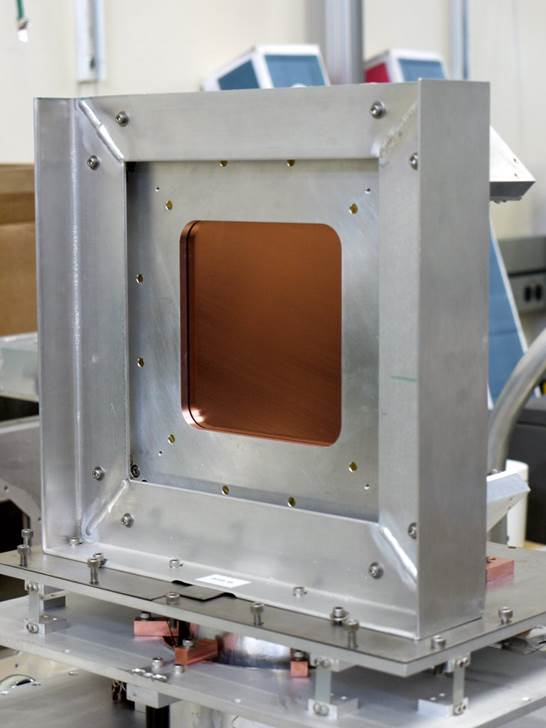
\includegraphics[width=2.25in]{../images/ch5-focal-plane-cryostat.jpg}};
    \begin{scope}[x={(image.south east)},y={(image.north west)}]
	    % \draw[help lines,xstep=.1,ystep=.1] (0,0) grid (1.0,1);
		% \foreach \x in {0,1,...,9} { \node [anchor=north] at (\x/10,0) {0.\x}; }
		% \foreach \y in {0,1,...,9} { \node [anchor=east] at (0,\y/10) {0.\y}; }
		
        \draw[black,ultra thick,rounded corners] (0.2,0.50) rectangle (0.10,0.70) node[below right] {\textbf{A}}; % T-box / frame
        \draw[black,ultra thick,rounded corners] (0.25,0.07) rectangle (0.12,0.15) node[below right] {\textbf{B}}; % 90-K cold plate
        
       \draw[black,ultra thick,<->] (.13,0.90) -- (0.82,0.90) node[midway,above] {xxx in}; % scale bar
    \end{scope}
\end{tikzpicture}

\end{document}
